%%%%%%%%%%%%%%%%%%%% book.tex %%%%%%%%%%%%%%%%%%%%%%%%%%%%%
%
% sample root file for the chapters of your "monograph"
%
% Use this file as a template for your own input.
%
%%%%%%%%%%%%%%%% Springer-Verlag %%%%%%%%%%%%%%%%%%%%%%%%%%


% RECOMMENDED %%%%%%%%%%%%%%%%%%%%%%%%%%%%%%%%%%%%%%%%%%%%%%%%%%%
\documentclass[graybox,envcountchap,sectrefs]{svmono}

% choose options for [] as required from the list
% in the Reference Guide

\usepackage{mathptmx}
\usepackage{helvet}
\usepackage{courier}
%
\usepackage{type1cm}         

\usepackage{makeidx}         % allows index generation
\usepackage[pdftex]{graphicx}        % standard LaTeX graphics tool
                             % when including figure files
\usepackage{multicol}        % used for the two-column index
\usepackage[bottom]{footmisc}% places footnotes at page bottom

% see the list of further useful packages
% in the Reference Guide

\makeindex             % used for the subject index
                       % please use the style svind.ist with
                       % your makeindex program

%%%%%%%%%%%%%%%%%%%%%%%%%%%%%%%%%%%%%%%%%%%%%%%%%%%%%%%%%%%%%%%%%%%%%

\begin{document}

\author{Author name(s)}
\title{Book title}
\subtitle{-- Monograph --}
\maketitle

\frontmatter%%%%%%%%%%%%%%%%%%%%%%%%%%%%%%%%%%%%%%%%%%%%%%%%%%%%%%


%%%%%%%%%%%%%%%%%%%%%%% dedic.tex %%%%%%%%%%%%%%%%%%%%%%%%%%%%%%%%%
%
% sample dedication
%
% Use this file as a template for your own input.
%
%%%%%%%%%%%%%%%%%%%%%%%% Springer %%%%%%%%%%%%%%%%%%%%%%%%%%

\begin{dedication}
Use the template \emph{dedic.tex} together with the Springer document class SVMono for monograph-type books or SVMult for contributed volumes to style a quotation or a dedication\index{dedication} at the very beginning of your book in the Springer layout
\end{dedication}





%%%%%%%%%%%%%%%%%%%%%%foreword.tex%%%%%%%%%%%%%%%%%%%%%%%%%%%%%%%%%
% sample foreword
%
% Use this file as a template for your own input.
%
%%%%%%%%%%%%%%%%%%%%%%%% Springer %%%%%%%%%%%%%%%%%%%%%%%%%%

\foreword

%% Please have the foreword written here
Use the template \textit{foreword.tex} together with the Springer document class SVMono (monograph-type books) or SVMult (edited books) to style your foreword\index{foreword} in the Springer layout. 

The foreword covers introductory remarks preceding the text of a book that are written by a \textit{person other than the author or editor} of the book. If applicable, the foreword precedes the preface which is written by the author or editor of the book.


\vspace{\baselineskip}
\begin{flushright}\noindent
Place, month year\hfill {\it Firstname  Surname}\\
\end{flushright}



%%%%%%%%%%%%%%%%%%%%%%preface.tex%%%%%%%%%%%%%%%%%%%%%%%%%%%%%%%%%%%%%%%%%
% sample preface
%
% Use this file as a template for your own input.
%
%%%%%%%%%%%%%%%%%%%%%%%% Springer %%%%%%%%%%%%%%%%%%%%%%%%%%

\preface

%% Please write your preface here
Use the template \emph{preface.tex} together with the Springer document class SVMono (monograph-type books) or SVMult (edited books) to style your preface in the Springer layout.

A preface\index{preface} is a book's preliminary statement, usually written by the \textit{author or editor} of a work, which states its origin, scope, purpose, plan, and intended audience, and which sometimes includes afterthoughts and acknowledgments of assistance. 

When written by a person other than the author, it is called a foreword. The preface or foreword is distinct from the introduction, which deals with the subject of the work.

Customarily \textit{acknowledgments} are included as last part of the preface.
 

\vspace{\baselineskip}
\begin{flushright}\noindent
Place(s),\hfill {\it Firstname  Surname}\\
month year\hfill {\it Firstname  Surname}\\
\end{flushright}



%%%%%%%%%%%%%%%%%%%%%%acknow.tex%%%%%%%%%%%%%%%%%%%%%%%%%%%%%%%%%%%%%%%%%
% sample acknowledgement chapter
%
% Use this file as a template for your own input.
%
%%%%%%%%%%%%%%%%%%%%%%%% Springer %%%%%%%%%%%%%%%%%%%%%%%%%%

\extrachap{Acknowledgements}

Use the template \emph{acknow.tex} together with the Springer document class SVMono (monograph-type books) or SVMult (edited books) if you prefer to set your acknowledgement section as a separate chapter instead of including it as last part of your preface.



\tableofcontents

%%%%%%%%%%%%%%%%%%%%%%acronym.tex%%%%%%%%%%%%%%%%%%%%%%%%%%%%%%%%%%%%%%%%%
% sample list of acronyms
%
% Use this file as a template for your own input.
%
%%%%%%%%%%%%%%%%%%%%%%%% Springer %%%%%%%%%%%%%%%%%%%%%%%%%%

\extrachap{Acronyms}

Use the template \emph{acronym.tex} together with the Springer document class SVMono (monograph-type books) or SVMult (edited books) to style your list(s) of abbreviations or symbols in the Springer layout.

Lists of abbreviations\index{acronyms, list of}, symbols\index{symbols, list of} and the like are easily formatted with the help of the Springer-enhanced \verb|description| environment.

\begin{description}[CABR]
\item[ABC]{Spelled-out abbreviation and definition}
\item[BABI]{Spelled-out abbreviation and definition}
\item[CABR]{Spelled-out abbreviation and definition}
\end{description}


\mainmatter%%%%%%%%%%%%%%%%%%%%%%%%%%%%%%%%%%%%%%%%%%%%%%%%%%%%%%%
%%%%%%%%%%%%%%%%%%%%%part.tex%%%%%%%%%%%%%%%%%%%%%%%%%%%%%%%%%%
% 
% sample part title
%
% Use this file as a template for your own input.
%
%%%%%%%%%%%%%%%%%%%%%%%% Springer %%%%%%%%%%%%%%%%%%%%%%%%%%

\begin{partbacktext}
\part{Part Title}
\noindent Use the template \emph{part.tex} together with the Springer document class SVMono (monograph-type books) or SVMult (edited books) to style your part title page and, if desired, a short introductory text (maximum one page) on its verso page in the Springer layout.

\end{partbacktext}
%%%%%%%%%%%%%%%%%%%%% chapter.tex %%%%%%%%%%%%%%%%%%%%%%%%%%%%%%%%%
%
% sample chapter
%
% Use this file as a template for your own input.
%
%%%%%%%%%%%%%%%%%%%%%%%% Springer-Verlag %%%%%%%%%%%%%%%%%%%%%%%%%%
%\motto{Use the template \emph{chapter.tex} to style the various elements of your chapter content.}
\chapter{Introduction}
\label{introduction} % Always give a unique label
% use \chaptermark{}
% to alter or adjust the chapter heading in the running head

\abstract*{As one of the key areas that appeals directly to the majority of the human race, Virtual Reality is receiving a high level of attention at present. Despite this, there is still much space for growth within the field for navigation frameworks. In this chapter, We introduce our framework by defining the problem we seek to address. Details regarding importance of this project and the necessary background details, including relevant details from industry projects, are succinctly summarized. An analysis of existing industrial trends pertaining to VR included as well. The scope of the project is defined along with the expected outcomes. Research outcomes expected from this project are described in considerable depth with the hope of providing a clear outline of the scientific contribution of the project.}

\abstract{As one of the key areas that appeals directly to the majority of the human race, Virtual Reality is receiving a high level of attention at present. Despite this, there is still much space for growth within the field for navigation frameworks. In this chapter, We introduce our framework by defining the problem we seek to address. Details regarding importance of this project and the necessary background details, including relevant details from industry projects, are succinctly summarized. An analysis of existing industrial trends pertaining to VR included as well. The scope of the project is defined along with the expected outcomes. Research outcomes expected from this project are described in considerable depth with the hope of providing a clear outline of the scientific contribution of the project.}

\section{Problem Background}
\label{sec:1}

The concept of Virtual Reality first emerged during 1950s and experiencing Virtual Reality using a head mounted display system wasn?t introduced during late 1960s. With the advances in the field of generation of 3D content and image processing, this topic caught the interest of many and the recent release of Oculus RIFT, SamsaungVR gear and especially Google Cardboard as an inexpensive alternative, the field is once again in the limelight. However generating content for virtual reality applications still remains to be a technically challenging and expensive task. Thus Virtual Reality is still a cutting edge technology with a great deal of unexplored potential.

Currently VR technologies are mostly used for games, to create an immersive experience within a computer generated environment. The few uses of real world content account to the fact that the content generation process requires dedicated hardware and proprietary software, but even with that the generated environment is immensely restrictive. Therefore mass scale applications utilizing VR technologies are almost non-existent.

However, the use of Virtual Reality in the fields of Medicine, Education, and Media etc... Is being explored and researched by scholars and it has emerged as a very promising technology. Hence, VR could be stated to be one of the timeliest areas for research and development in.

\section{Importance of the Problem}
\label{intro_sec:2}
% Always give a unique label
% and use \ref{<label>} for cross-references
% and \cite{<label>} for bibliographic references
% use \sectionmark{}
% to alter or adjust the section heading in the running head

\subsection{Growth of Industry}
\label{intro_subsec:2_1}

Virtual Reality is becoming the future of immersion for computer generated imagery. As the following business insider graph predicts, the shift to virtual reality is increasing drastically.

\begin{figure}[htbp]
\begin{center}
\includegraphics[width=\textwidth]{Figures/1.png}
\caption{Global Virtual Reality Head-Mounted Display Shipments \cite{1}}
\label{fig1_1}
\end{center}
\end{figure}


With the increase of availability of the virtual reality hardware, the market potential of VR has a significant importance. The graph below shows the percentage of income from VR in different areas.

Therefore the greater part of VR revenue will depend on the software solutions available to exploit the shift to VR. This is evident by many start-ups forming to take advantage of this market niche such as, Jaunt VR \cite{4}, Vahana VR \cite{5}, Samsung LiveLife \cite{6}, HP ZVR \cite{7}.

Not only start-ups, all the big players in the industry have started investing heavily on virtual reality technologies. This is evident through projects such as Google Cardboard project \cite{2} which aims to make virtual reality accessible at a low cost, Microsoft?s Hololense \cite{8}. Even Facebook has joined up the VR hype by acquiring the Oculus which was the leading virtual reality headband producer at the time.

\begin{figure}[htbp]
\begin{center}
\includegraphics[width=\textwidth]{Figures/2.png}
\caption{Augmented and Virtual Reality To Hit \$150 Billion \cite{3}}
\label{fig1_2}
\end{center}
\end{figure}

With these new trends a significant reduction of cost can be seen for Virtual reality hardware. Unlike the old days, anyone who owns a smartphone may convert it to a virtual reality head band with the google cardboard at a very low cost. With this drastic reduction in cost virtual reality is accessible by any person. However the content creation remains a high costly process requiring specialized equipment. This is a barrier this project aims to eliminate.

\subsection{Applications Utilizing VR}
\label{intro_subsec:2_2}

This new trend in virtual reality has helped in many professions and fields. For an example in the medical industry \cite{9}. The special use cases in surgery is discussed in this paper \cite{10}. The use of VR in therapy and rehabilitation is another use case for this technology. 

Man, mind, and machine: the past and future of virtual reality simulation in neurologic surgery discusses the use of VR in neurologic surgery \cite{11}.

Other than the medical field there are uses in Virtual reality technologies in education, training and marketing areas as well which are elaborated in Immersive training systems: Virtual Reality and Education and Training \cite{12} and  The Effects of Virtual Reality on Consumer Learning (Marketing) \cite{13}.

\subsection{Space for Improvement}
\label{intro_subsec:2_3}

The project will focus greatly on the underlying algorithms for creating content as well as rendering content. In order to successfully use low cost smartphones and cameras, and give an immersive experience through virtual reality these algorithms need to be optimised to use the least amount of resources.

Thus by analysing image stitching, video stitching and rendering algorithms and optimising them for the use on mobile phones with their inherent limitations in computational power and memory, the project will have huge impact on making VR technology widely available.

This contribution of the project will give the required core software backing to complete the transition of virtual reality from unaffordable to affordable.

\section{Scope of the Project}
\label{intro_sec:3}

The project work plans to deliver a significant contribution to the scientific research in the fields in Computer Vision, Image Processing, Virtual Reality, and other related fields.

Major contributions from the project has been identified as the following:

\begin{itemize}
\item{An evaluation of Image Stitching Algorithms}
\item{A mathematical model for generating intermediate spheres}
\item{An optimization strategy for streaming immersive VR over a network}
\item{A Scene Description Language for representing Navigable VR environments}
\item{Intuitive gesture system based on a Machine Learning Algorithm}
\item{A four-camera rig which aligns itself with the compass direction}
\end{itemize}

\subsection{An Evaluation of Image Stitching Algorithms}
\label{intro_subsec:3_1}

The first stage of the project would be to analyse existing algorithms for Image stitching algorithms. After conducting a thorough literature survey, several Image stitching algorithms, including the following will be chosen for testing.

\begin{itemize}
\item{Fast panorama stitching for high-quality panoramic images on mobile phones \cite{14}}
\item{Automatic Panorama Image Stitching using Invariant Features \cite{15}}
\item{Video Stitch Algorithm Based on Dynamic Foreground Extraction \cite{16}}
\item{Efficient Video Panoramic Image Stitching Based on an Improved Selection of Harris Corners and a Multiple-Constraint Corner Matching \cite{17}}
\item{Stitching Video from Webcams}
\end{itemize}

A testing framework will be developed to assess the qualitative aspects as well as quantitative aspects of the each algorithm. The colour correction and the structure of the stitched image would be taken into account for this testing.

\paragraph{Expected Outcomes}
\begin{itemize}
\item{Implementation of image stitching techniques described in the selected research papers.}
\item{Testing framework for image stitching.}
\item{Evaluation method for image stitching algorithms capturing both qualitative and quantitative aspects.}
\end{itemize}

\paragraph{Deliverables}
\begin{itemize}
\item{Research paper evaluating selected image stitching algorithms.}
\end{itemize}
The paper will present the testing framework and the test results, and differentiate each algorithm and identify their strong points and weaknesses which will help to choose the best algorithm for the project.

\subsection{Image Sphere}
\label{intro_subsec:3_2}

The next phase of the project is to create the image sphere using a set of images. Using the selected image stitching algorithm from the previous phase a panorama of the full 360 x 360 degree images will be created. 

In order to use this stitched panorama it will be projected onto a sphere, several methods for projecting a 2D panorama into a sphere will be considered along with the representation of these for rendering.

\paragraph{Expected Outcomes}
\begin{itemize}
\item{Storing image spheres in a portable format.}
\item{Rendering image spheres in google cardboard app.}
\end{itemize}

\paragraph{Deliverables}
\begin{itemize}
\item{PoC system for stitching and viewing 360 images}
\end{itemize}

\subsection{Navigation in a Static Environment}
\label{intro_subsec:3_3}

After the image stitching and projection on a sphere is complete we would look at giving the user a more immersive experience by making it possible to navigate through the environment. This would be done by creating image spheres as the point of view changes using the available image sphere data.

Our target will be to adopt this technique and improve it keeping in mind the constraints imposed when we use smartphones as the device to run our application.

Moreover, in order to make the traversal process less time consuming, an environment map will be pre-generated, and stored in a Scene Description Language (SDL) embedded into the image spheres.

\paragraph{Expected Outcomes}
\begin{itemize}
\item{Navigation in-between Static 360$^{\circ}$$\times$360$^{\circ}$ panoramic images.}
\end{itemize}

\paragraph{Deliverables}
\begin{itemize}
\item{A Scene Description Language (SDL) for navigation in static panoramic image environments.}
\item{A mathematical model for intermediate sphere generation.}
\item{Research paper on the navigation technique and final outcome of the project.}
\end{itemize}

\subsection{Immersive and Intuitive Gesture-based Navigation}
\label{intro_subsec:3_4}

When the environment itself is fully navigable, and the user is able to experience the immersive reality with minimal restrictions, the remaining question will be the method of navigation.

Walking around is not practical as physical movements while wearing a VR headgear is bound to be dangerous to the person. A button based input system is unsophisticated as it will be ruining the immersive experience of the user. Hence as a solution we would explore the possibilities of implementing an intuitive gesture, which is practical and supportive to the illusion of immersiveness.

\paragraph{Expected Outcomes}
\begin{itemize}
\item{The user is able to freely navigate within the immersive environment.}
\end{itemize}

\paragraph{Deliverables}
\begin{itemize}
\item{An intuitive gesture input system for navigation inside a virtual environment}
\item{Research paper on the intuitive gesture recognition system}
\end{itemize}

\subsection{Optimization Strategy for Streaming VR Content}
\label{intro_subsec:3_5}

By nature, VR content requires a lot of information. Thus, streaming VR content over a network necessitates more data. But, for a user immersed in a virtual world, all the details are not important, as the Field of View of is quite narrow. However, just streaming the data attached to the viewpoint is not feasible as a user making a sudden movement will require different areas of vision.

Our research work aims to find a suitable mechanism to allow the users to have an immersive experience while making sure the data flow over the network is minimal. Possible solutions include, differentiating the quality of streamed data, and predicting user movements, etc..

\paragraph{Expected Outcomes}
\begin{itemize}
\item{The system is able to stream VR data with minimal data consumption.}
\end{itemize}

\paragraph{Deliverables}
\begin{itemize}
\item{An optimization algorithm for streaming VR content over a network.}
\end{itemize}

\subsection{Multi-camera Rig for Panoramic Image Capture}
\label{intro_subsec:3_6}

In order to generate panoramas, it is not practical to acquire individual photos and send them into a stitching process to obtain it. Thus, one of the objectives in this research work is to create a multi camera rig, specially designed to capture panoramas, along with location data for environment generation \cite{18}. 

Also, the camera rig needs to be equipped with a self-adjusting feature to align itself to the same compass direction for taking panoramic photos in the same series. This is in order to make aligning the panoramas without further calculations.

\paragraph{Expected Outcomes}
\begin{itemize}
\item{The user is able to capture photos from a camera rig, without worrying about technical details.}
\end{itemize}

\paragraph{Deliverables}
\begin{itemize}
\item{A physical four-camera rig, self-adjusting to the same compass direction.}
\end{itemize}

\section{Coverage of Research Areas}
\label{intro_sec:4}

As a project that involves mapping real world scenarios to virtual environments and allowing visualization using Virtual Reality, this project covers several key research areas in computer science.

Primary among these are,
\begin{enumerate}
\item{Image Processing}
\item{Computer Vision}
\item{Computer Graphics}
\item{Human Computer Interaction}
\item{Machine Learning}
\end{enumerate}

\paragraph{Image Processing}
%\label{intro_subsec:4_1}
As a framework for creating VR content using image input, the pre-processing steps used in images at various steps form a crucial part of the system. These include grey scaling, applying various filters, edge detection and colour correction.

\paragraph{Computer Vision}
%\label{intro_subsec:4_2}
In creating a panoramic image using individual images, image stitching is especially important. In performing stitching, feature extraction and correlation form the very basis of correlating matching parts of separate images together.

\paragraph{Computer Graphics}
%\label{intro_subsec:4_3}
Projecting the stitched panorama into a sphere and additionally providing an intuitive visualization of the sphere using a game engine falls under the category of Computer Graphics.

\paragraph{Human Computer Interaction}
%\label{intro_subsec:4_4}
Using a VR headset for navigation is not inherently intuitive. As the interactivity of the scene is increased, providing an intuitive navigation framework becomes harder. Suggesting a seamless navigation method which provides a smooth experience for the viewer is very important to the overall goal of ensuring immersiveness.

\paragraph{Machine Learning}
%\label{intro_subsec:4_5}
Navigating using gestures provides its own challenge of recognizing said gestures. A machine learning based approach is considered in this regard so as to ensure the maximum accuracy along with very high responsiveness.

%%%%%%%%%%%%%%%%%%%%% appendix.tex %%%%%%%%%%%%%%%%%%%%%%%%%%%%%%%%%
%
% sample appendix
%
% Use this file as a template for your own input.
%
%%%%%%%%%%%%%%%%%%%%%%%% Springer-Verlag %%%%%%%%%%%%%%%%%%%%%%%%%%

\appendix
\motto{All's well that ends well}
\chapter{Chapter Heading}
\label{introA} % Always give a unique label
% use \chaptermark{}
% to alter or adjust the chapter heading in the running head

Use the template \emph{appendix.tex} together with the Springer document class SVMono (monograph-type books) or SVMult (edited books) to style appendix of your book in the Springer layout.


\section{Section Heading}
\label{sec:A1}
% Always give a unique label
% and use \ref{<label>} for cross-references
% and \cite{<label>} for bibliographic references
% use \sectionmark{}
% to alter or adjust the section heading in the running head
Instead of simply listing headings of different levels we recommend to let every heading be followed by at least a short passage of text. Furtheron please use the \LaTeX\ automatism for all your cross-references and citations.


\subsection{Subsection Heading}
\label{sec:A2}
Instead of simply listing headings of different levels we recommend to let every heading be followed by at least a short passage of text. Furtheron please use the \LaTeX\ automatism for all your cross-references and citations as has already been described in Sect.~\ref{sec:A1}.

For multiline equations we recommend to use the \verb|eqnarray| environment.
\begin{eqnarray}
\vec{a}\times\vec{b}=\vec{c} \nonumber\\
\vec{a}\times\vec{b}=\vec{c}
\label{eq:A01}
\end{eqnarray}

\subsubsection{Subsubsection Heading}
Instead of simply listing headings of different levels we recommend to let every heading be followed by at least a short passage of text. Furtheron please use the \LaTeX\ automatism for all your cross-references and citations as has already been described in Sect.~\ref{sec:A2}.

Please note that the first line of text that follows a heading is not indented, whereas the first lines of all subsequent paragraphs are.

% For figures use
%
\begin{figure}[t]
\sidecaption[t]
%\centering
% Use the relevant command for your figure-insertion program
% to insert the figure file.
% For example, with the option graphics use
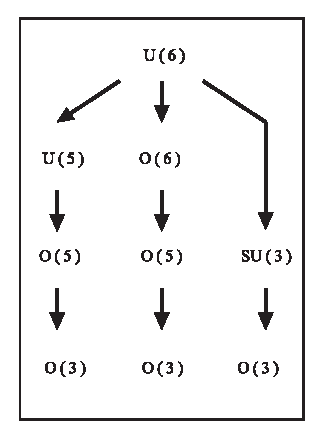
\includegraphics[scale=.65]{figure}
%
% If not, use
%\picplace{5cm}{2cm} % Give the correct figure height and width in cm
%
\caption{Please write your figure caption here}
\label{fig:A1}       % Give a unique label
\end{figure}

% For tables use
%
\begin{table}
\caption{Please write your table caption here}
\label{tab:A1}       % Give a unique label
%
% For LaTeX tables use
%
\begin{tabular}{p{2cm}p{2.4cm}p{2cm}p{4.9cm}}
\hline\noalign{\smallskip}
Classes & Subclass & Length & Action Mechanism  \\
\noalign{\smallskip}\hline\noalign{\smallskip}
Translation & mRNA$^a$  & 22 (19--25) & Translation repression, mRNA cleavage\\
Translation & mRNA cleavage & 21 & mRNA cleavage\\
Translation & mRNA  & 21--22 & mRNA cleavage\\
Translation & mRNA  & 24--26 & Histone and DNA Modification\\
\noalign{\smallskip}\hline\noalign{\smallskip}
\end{tabular}
$^a$ Table foot note (with superscript)
\end{table}
%


\backmatter%%%%%%%%%%%%%%%%%%%%%%%%%%%%%%%%%%%%%%%%%%%%%%%%%%%%%%%
%%%%%%%%%%%%%%%%%%%%%%acronym.tex%%%%%%%%%%%%%%%%%%%%%%%%%%%%%%%%%%%%%%%%%
% sample list of acronyms
%
% Use this file as a template for your own input.
%
%%%%%%%%%%%%%%%%%%%%%%%% Springer %%%%%%%%%%%%%%%%%%%%%%%%%%

\Extrachap{Glossary}


Use the template \emph{glossary.tex} together with the Springer document class SVMono (monograph-type books) or SVMult (edited books) to style your glossary\index{glossary} in the Springer layout.


\runinhead{glossary term} Write here the description of the glossary term. Write here the description of the glossary term. Write here the description of the glossary term.

\runinhead{glossary term} Write here the description of the glossary term. Write here the description of the glossary term. Write here the description of the glossary term.

\runinhead{glossary term} Write here the description of the glossary term. Write here the description of the glossary term. Write here the description of the glossary term.

\runinhead{glossary term} Write here the description of the glossary term. Write here the description of the glossary term. Write here the description of the glossary term.

\runinhead{glossary term} Write here the description of the glossary term. Write here the description of the glossary term. Write here the description of the glossary term.

\Extrachap{Solutions}

\section*{Problems of Chapter~\ref{intro}}

\begin{sol}{prob1}
The solution\index{problems}\index{solutions} is revealed here.
\end{sol}


\begin{sol}{prob2}
\textbf{Problem Heading}\\
(a) The solution of first part is revealed here.\\
(b) The solution of second part is revealed here.
\end{sol}


\printindex

%%%%%%%%%%%%%%%%%%%%%%%%%%%%%%%%%%%%%%%%%%%%%%%%%%%%%%%%%%%%%%%%%%%%%%

\end{document}





